\documentclass{article}
\usepackage{arxiv}
\setcounter{secnumdepth}{2} 
\fancyfoot{}
\sloppy
\usepackage{wrapfig}
\usepackage{booktabs} % For formal tables
\usepackage{caption}
\usepackage{subcaption}
\usepackage{amsmath,amssymb,amsfonts}
\usepackage{algorithmic}
\usepackage[numbers]{natbib}
\usepackage{comment}
\usepackage[linesnumbered,ruled,vlined]{algorithm2e}
\SetKwComment{Comment}{$\triangleright$\ }{}
\usepackage{graphicx}
\usepackage{textcomp}
\usepackage{multirow}
\usepackage{hyperref}
\usepackage[table, svgnames, dvipsnames]{xcolor}
\usepackage{makecell, cellspace, caption}
\def\BibTeX{{\rm B\kern-.05em{\sc i\kern-.025em b}\kern-.08em
    T\kern-.1667em\lower.7ex\hbox{E}\kern-.125emX}}

\def\A{{\bf A}}
\def\a{{\bf a}}
\def\B{{\bf B}}
\def\b{{\bf b}}
\def\C{{\bf C}}
\def\c{{\bf c}}
\def\D{{\bf D}}
\def\d{{\bf d}}
\def\E{{\bf E}}
\def\e{{\bf e}}
\def\F{{\bf F}}
\def\f{{\bf f}}
\def\g{{\bf g}}
\def\h{{\bf h}}
\def\G{{\bf G}}
\def\H{{\bf H}}
\def\I{{\bf I}}
\def\K{{\bf K}}
\def\k{{\bf k}}
\def\l{{\bf l}}
\def\M{{\bf M}}
\def\m{{\bf m}}
\def\N{{\bf N}}
\def\n{{\bf n}}
\def\Q{{\bf Q}}
\def\q{{\bf q}}
\def\R{{\bf R}}
\def\S{{\bf S}}
\def\s{{\bf s}}
\def\T{{\bf T}}
\def\U{{\bf U}}
\def\u{{\bf u}}
\def\V{{\bf V}}
\def\v{{\bf v}}
\def\W{{\bf W}}
\def\w{{\bf w}}
\def\X{{\bf X}}
\def\x{{\bf x}}
\def\Y{{\bf Y}}
\def\y{{\bf y}}
\def\Z{{\bf Z}}
\def\z{{\bf z}}
\def\0{{\bf 0}}
\def\1{{\bf 1}}
\def\RB{{\mathbb R}}

\newcommand{\red}[1]{{\color{red}#1}}

\title{CS 584: Sentence Similarity Classifier} % \\

\author{
% suggested author list, if you work with another student, provide names and email addresses for both.
Jonathan Pruchansky\textsuperscript{*}\\
\textsuperscript{*}{Stevens Institute of Technology}\\
jpruchan@stevens.edu\\
Spring 2025
}
\date{\today}
\begin{document}
\maketitle
\begin{abstract}
A standard problem in NLP is the process of identifying semantic similarity between different sentences. This problem is applicable in several contexts, with online forums or machine translation being some notable examples. In general, this problem is useful in any context where one would like to evaluate similarity between sentences, whether it's a means to evaluate the performance of a larger project, or as simple as classifying redundant web pages. This problem will be approached by developing a neural network that works with SkipGram word embeddings to derive contextual meaning from words within sentences to identify semantic similarity.
\end{abstract}

% Include the sections you need to present
\section{Introduction}
The problem of classifying different sentences as semantically similar is important in many contexts. For example, online forums would like to make sure their websites avoid duplicate threads with slightly different questions that ask the same thing. It's also a good way to evaluate NLP tasks like machine translation. What's the best way to check if a translation is accurate? To check if the meaning of the sentence is retained through translation. One can use a sematic similarity test on the original sentence compared to a sentence that was translated to a different language and then back. The scope of this project is to create a basic tool that, given two sentences, tells the user a yes or no answer to the question: Are these two sentences trying to convey the same meaning? The final goal is to develop a tool that allows users to compare words, sentences, and maybe even paragraphs based on how closely their meanings align with each other.
\section{Related Work}
The drive for this kind of technology comes from online message forums such as Quora. They maintain that their website runs on the principle that "there should be a single question page for each logically distinct question"(Csernai). Kornél Csernai, who is a Machine Learning Platform Engineer at Quora, says that their company is "always searching for a better solution" to this problem (Csernai). A paper published in May of 2022 by researchers from MIT addresses two main challenges in classifying sematic similarity. The first being a lack of sufficient labeled data and the other being the train-test gap of calculating inter-sentence semantic scores (Sun). This project will aim to combat the first issue using a dataset with over 400,000 entries of labeled data, significantly larger than the 8,628 data points used by Sun and the other authors.

\section{Methodology}
To formulate the problem in terms of a model, given two sentences as input, we output a number 0 or 1 to determine whether or not the two sentences are semantically similar. First, the sentences will be converted to vector format using SkipGram word embeddings. These embeddings will be sourced from Assignment 2. This set of embeddings encompasses a vocab of over 100,000 words. The reason we use pretrained embeddings is to simplify to the task to be purely classification as opposed to learning both embeddings and similarity between sentences at the same time. This will bring down training time significantly, and will avoid recomputing word embeddings that we already have available.
\begin{figure}[htp]
    \centering
    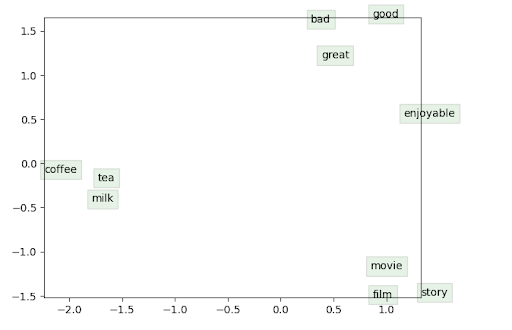
\includegraphics[width=10cm]{embeddings.png}
    \caption{Implicit evaluation of the word embeddings}
\end{figure}

The figure above shows that the word embeddings that were computed in assignment 2 do a great job of grasping semantic similarity between different words. Words that are synonyms or share some sort of context like good and great or film and movie are grouped together in this projection. This is perfect for application in an external task where semantic context is important.

\subsection{Approach 1: Feed Forward Network}
The first approach that was tested was a simple fully connected feed forward network. This network consisted of two RELU hidden layers of size 256 and 64 followed by an output layer of size 1 with sigmoid activation.
\begin{figure}[htp]
    \centering
    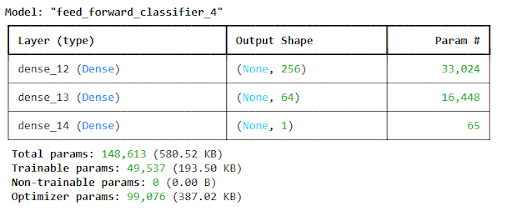
\includegraphics[width=10cm]{model1.png}
    \caption{Model 1 Architecture}
\end{figure}
In order to pass input to this model, we have to find a way to represent each sentence as a vector of fixed length. A common approach, that was used for this model, is to take the average of each word vector in the sentence. Finally, the two vector forms of the sentences are concatenated and fed into the neural network. This model was trained with the classic binary cross entropy loss. The following figure displays some of the statistics from the training process.
\begin{figure}[htp]
    \centering
    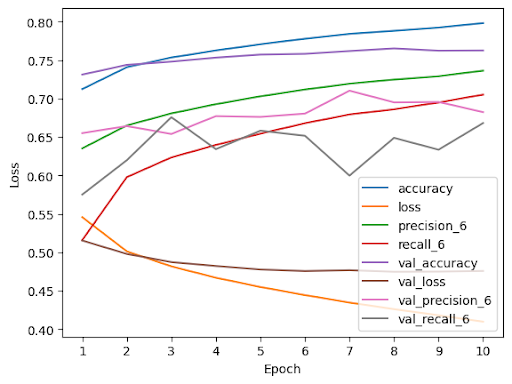
\includegraphics[width=10cm]{model1_train.png}
    \caption{Model 1 Training Process}
\end{figure}
There are a few important takeaways from this training process. For one, the training loss and the validation loss are both being driven downward at a steady rate. This means that the model is successfully learning the training data while generalizing enough to perform well on a potential test set. Additionally, all metrics both for the training and validation data are consistently going up which means the model is improving in performance. The results of evaluating this model on the test set will be discussed in a later section along with the other models.

\subsection{Approach 2: LSTM with Cosine Similarity}
The first model works great and all, but taking the average of every word embedding in the sentence may not be the best way to represent its semantic meaning. Instead, it's possible to learn a good vectorized representation for each sentence. This is achieved through an LSTM bidirectional recurrent neural network that will generate a semantic "context" for a given sentence.
\begin{figure}[htp]
    \centering
    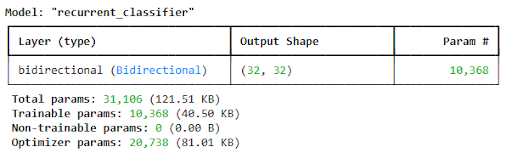
\includegraphics[width=10cm]{model2.png}
    \caption{Model 2 Architecture}
\end{figure}
This works well because the RNN can take in a sentence of any length and output a fixed sized. This is the problem that was solved by taking an average for the previous model. Now, this allows us to have a learned representation of each sentence instead of a presupposed one. After we generate the "context" for both sentences, we compare the context vectors using cosine similarity. If the similarity between the context vectors is greater than 0, this means the sentences are semantically similar, otherwise they are not. In hindsight, this may not have been the best decision, and this will be addressed in a later section. As shown in the following figures, the model did not respond well to using binary cross entropy loss to evaluate the model. The loss was not decreasing throughout the training process, and the evaluation metrics remained unchanged during training. These shortcoming and other results from this model will be discussed in a later section in conjunction with the other models.
\begin{figure}[htp]
    \centering
    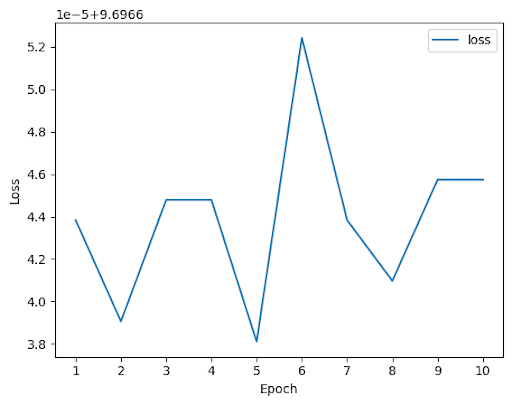
\includegraphics[width=7cm]{model2_train1.png}
    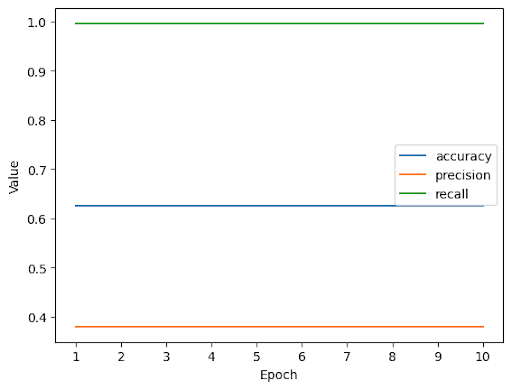
\includegraphics[width=7cm]{model2_train2.png}
    \caption{Model 2 Training Process}
\end{figure}

\subsection{Approach 3: Encoder Decoder}
The final model that we constructed was a multi step model with an "encoder" part and a "decoder" part.
\begin{figure}[htp]
    \centering
    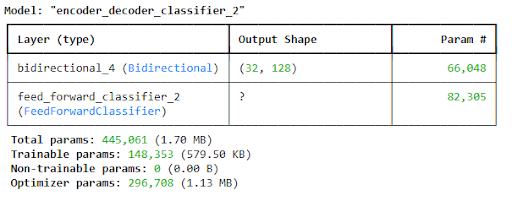
\includegraphics[width=10cm]{model3.png}
    \caption{Model 3 Architecture}
\end{figure}
This model takes the best attributes from the first two approaches and combines them into a single model. First, we take a given sentence and encode it into a fixed length context vector using the LSTM described in model 2. We do the same for the second input sentence. Then, instead of comparing the contexts using a predefined metric like a cosine similarity, we concatenate both context vectors and pass them through a feed forward net - the same network used in model 1. This allows the model to learn more complex similarity patterns in the encoded contexts. This part of the process is the "decoder" because it decodes any similarity between the given context vectors. This model responded significantly better to the training process. In fact, we argue that it responded a bit too well.
\begin{figure}[htp]
    \centering
    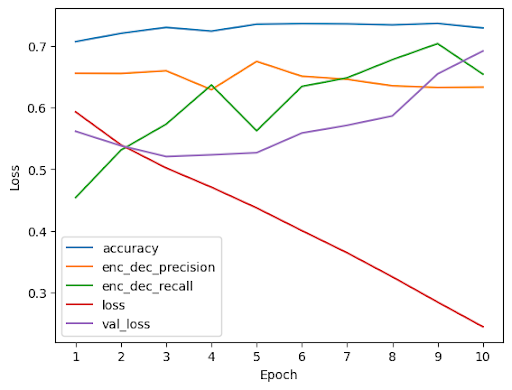
\includegraphics[width=10cm]{model3_train.png}
    \caption{Model 3 Training Process}
\end{figure}
The first thing to notice in the figure is that the training loss is consistently driven downward, which shows that the model is learning the training data well. However, after the first few epochs, the validation loss begins to increase. This means that the model is beginning to lose the ability to generalize well to unseen data, which can prove disastrous on a test set. Overall, the evaluation metrics for the training process are really good; in fact the accuracy went as high as 91 percent at one point (though the figure does not display this properly for some reason). Unfortunately, this did not translate well onto the testing set, and we discuss that in a following section.

\section{Experimental Setup}

\subsection{Data}
Since this problem is so important to Quora, they have provided a public, labeled dataset with questions from their website. Each entry in the set contains ids along with 2 sentences and a boolean indicator (1 or 0) if the two sentences are similar or not.
\subsection{Evaluation Metrics}
Since the project will be using a neural network to classify sentences as similar or not, the evaluation metrics that will be used are accuracy, precision, f1 score, and recall.
\subsection{Comparison Methods}
All of these approaches were tested and compared using binary cross entropy loss, accuracy, precision, and recall to see which offers the best solution to the problem. The following section details the results as well as the pros and cons of each approach.

\section{Results}
After evaluating each of the three models on a test set, we calculate and record each of the metrics for every model and output the results in the figure below.
\begin{figure}[htp]
    \centering
    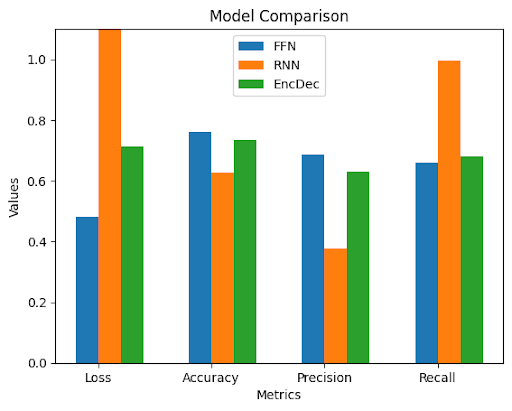
\includegraphics[width=10cm]{results.png}
    \caption{Model Results}
\end{figure}
The first thing to point out is that the feed forward network has the best overall results - best loss, accuracy, and precision. This is a very surprising result because it is definitely the simplest approach and required the least amount of designing, planning, and coding. Another point is that model 3, which is by far the most robust model, suffered a severe drop in performance compared to its results during training. This is a result of the overfitting that was mentioned in the previous section. It's possible that adding an attention mechanism to the encoder and adding dropout and batch normalization to the decoder will solve this pitfall. This is something that is still open to future testing. Finally, it's quite interesting that model 2 has such a high recall despite performing quite poorly in every other category. The reason for this may be the way the threshold for the cosine similarity was set. In the current design, if the cosine similarity between the context vectors is positive, then they are labeled as similar. This makes it really easy for the model to predict positive instances. Any slight similarity between sentences is instantly picked up on and labeled accordingly. A potential redesign is making the threshold for similarity a trainable parameter. This could allow the model to learn where the bound is between somewhat similar but slightly different contexts compared to 100 percent the same contexts. For now however, the best overall model remains the simple feedforward neural net, but with future improvements it's possible that the encoder decoder architecture may overcome the overfitting that currently drags it down.
\begin{footnotesize}
\bibliographystyle{plainnat}
\bibliography{ref}
Csernai, Kornél. "First Quora Dataset Release: Question Pairs". https://quoradata.quora.com/First-Quora-Dataset-Release-Question-Pairs
\newline
Sun, Xiaofei et al. Sentence Similarity Based on Contexts. https://direct.mit.edu/tacl/article/doi/10.1162/tacl\_a\_00477/111218/Sentence-Similarity-Based-on-Contexts
\end{footnotesize}%
\end{document}
